In diesem Problem geht es darum mithilfe von Messwerten der Schattengröße und dem Gewicht eines Tieres zu bestimmen ob es ein Hase oder Wiesel ist.Man kann es graphisch vorstellen als würde man alle Messwerte in ein Diagramm eintragen und versuchen eine Gerade $y=mx+n$ zu finden die die Gruppen von Punkten trennt.
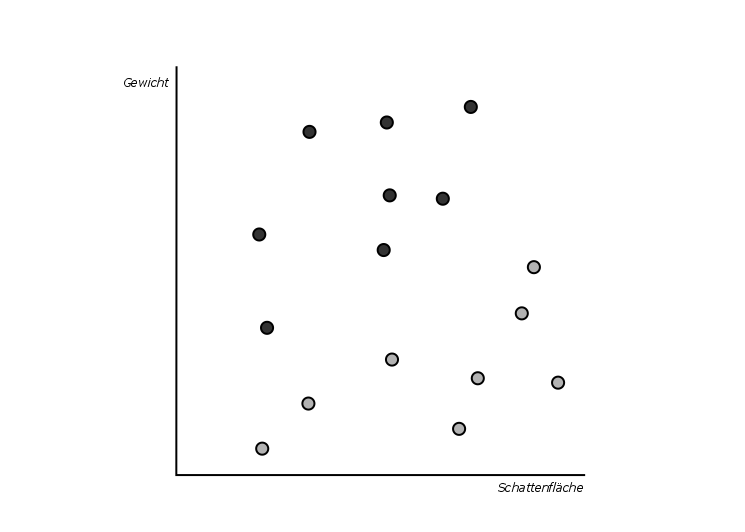
\includegraphics[width=\textwidth]{Grafiken/HaseWieselBild.png}
Dann würde gelten das \[y_h>mx_h+n\] für alle Hasen und \[
y_w<mx_w+n\] für alle Wiesel. Jedoch sind strikte Ungleichungen in linearen Programmen verboten. Deshalb wird eine Variable $\lambda$ eingeführt welche den Abstand zwischen allen Punkten und der Geraden beschreibt. Dies resultiert in den Ungleichungen:
\begin{align*}
	y_h\geq{}mx_h+n+\lambda\\
	y_w\leq{}mx_w+n-\lambda
\end{align*} 
Wobei versucht wird, $\lambda$ zu maximieren, ohne das Punkte auf der falschen Seite der Geraden liegen. Insgesamt ergibt sich das folgende lineare Programm:
\begin{alignat*}{3}
	\text{Maximiere }	   &&  \lambda&\\
	\text{so dass }&& y_h\geq{}mx_h+n+\lambda & \text{ für alle $h$}\\
				   &&y_w\leq{}mx_w+n-\lambda & \text{ für alle $w$}\\
\end{alignat*}
